\chapter{Avaliação e Testes}\label{cap:analise}

Este capítulo apresenta a execução prática da validação da solução proposta. Com base na metodologia e nas definições de ambiente (\textit{hardware}, \textit{software} e modelos de ML) detalhadas no \hyperref[cap:metodologia]{Capítulo~\ref*{cap:metodologia}}, esta seção foca em três aspectos centrais: a configuração do ambiente experimental, a comprovação da validação funcional e a análise comparativa de eficiência entre a solução em RL e a implementação nativa em C++. Por fim, serão apresentados os resultados obtidos durante os testes, acompanhados de uma análise crítica.

\section{Configuração do Ambiente Experimental}\label{sec:ambiente-experimental}

Para facilitar o processo de compilação e execução dos testes, foi estabelecido um ambiente de desenvolvimento padronizado. Um guia detalhado com o passo a passo para a instalação das ferramentas, compilação do compilador modificado e configuração das dependências encontra-se disponível no \hyperref[apendice:guia-instalacao]{Apêndice~\ref*{apendice:guia-instalacao}}.

A estrutura do projeto foi organizada de modo que os testes relacionados ao TFLM ficassem isolados no diretório \texttt{test/tflm-tests}. Neste diretório, foi alocado um \texttt{Makefile} personalizado, responsável por automatizar todo o processo de compilação, linkedição e execução dos testes.

Este \texttt{Makefile} executa as seguintes etapas principais para cada um dos arquivos de teste \texttt{.rob} presentes no diretório:
\begin{enumerate}
    \item Compila o código do \textit{wrapper} C do TFLM para gerar a biblioteca estática somente uma vez (caso ela não exista ou alguma configuração do \textit{wrapper} tenha sido modificada);
    \item Invoca o compilador Robcmp para traduzir os arquivos fonte \texttt{.rob} em código objeto (\textit{.o});
    \item Realiza a linkedição do código objeto gerado com as bibliotecas estáticas do TFLM (\texttt{libtensorflow-microlite.a}) e do \textit{wrapper} de compatibilidade desenvolvido.
    \item Executa todos os binários gerados, exibindo \textit{PASS} caso o retorno seja 0, ou \textit{FAILED} caso seja diferente de 0.
\end{enumerate}

Para garantir a otimização do tamanho do binário final e a compatibilidade com o TFLM em ambiente embarcado, foram utilizadas diversas \textit{flags} de compilação e linkedição. As principais opções adotadas e suas respectivas funções estão descritas a seguir:

\begin{description}
    \item[\texttt{-fno-rtti} e \texttt{-fno-exceptions}:] Desabilitam informações de tipo em tempo de execução e o suporte a exceções do C++ na compilação do \textit{wrapper}.
    \item[\texttt{-DTF\_LITE\_STATIC\_MEMORY=1}:] Define uma macro que instrui o TFLM a utilizar alocação de memória estática, o que é preferível em sistemas embarcados e necessário para compatibilidade com a RL.
    \item[\texttt{-ffunction-sections} e \texttt{-fdata-sections}:] Forçam o compilador a colocar cada função e item de dados em sua própria seção de memória.
    \item[\texttt{-Oz}:] Flag de compilação dos arquivos \texttt{.rob}. Nível de otimização agressivo focado na redução do tamanho do código gerado.
    \item[\texttt{-Wl,--gc-sections}:] Realiza a coleta de lixo (\textit{garbage collection}) de seções não utilizadas.
    \item[\texttt{-Wl,--strip-debug}:] Remove informações de depuração do binário final.
    \item[\texttt{-Wl,--discard-all}:] Descarta todas as seções não essenciais do binário final.
    \item[\texttt{-Wl,--build-id=none}:] Remove o identificador de build do binário final.
    \item[\texttt{-Wl,--relax}]: Permite ao \textit{linker} otimizar instruções e endereços para reduzir o tamanho do código final.
    \item[\texttt{-flto=thin}:] Habilita a Otimização em Tempo de Linkedição (\textit{Link Time Optimization}), permitindo que o otimizador analise o programa como um todo, e não apenas arquivo por arquivo.
\end{description}

O ambiente foi configurado para gerar executáveis compatíveis com a arquitetura \texttt{x86\_64}, permitindo a validação apenas na máquina de desenvolvimento.

\section{Resultados da Validação Funcional}
Todos os testes unitários relacionados ao TFLM estão localizados na pasta \texttt{\seqsplit{test/tflm-tests}}. Essa separação foi necessária pois o processo de linkedição dos programas que utilizam o TFLM é diferente dos programas convencionais, exigindo a inclusão da biblioteca estática do TFLM e do \textit{wrapper} C.

Dentro do diretório de testes desejado, basta executar o comando \texttt{make} para que todos os testes sejam compilados e executados automaticamente. Como convenção, os arquivos de teste que utilizam a nova sintaxe possuem o prefixo \texttt{syntax-}, enquanto os que utilizam a biblioteca padrão possuem o prefixo \texttt{lib-}.

Um arquivo de exemplo foi colocado no apêndice no final deste trabalho que realiza os testes unitários com o modelo de classificação de spam. O \hyperref[lst:teste-bib-rob]{Código~\ref*{lst:teste-bib-rob}} apresenta o arquivo \texttt{lib-spam.rob}, que utiliza a biblioteca padrão, todos os outros testes unitários com a biblioteca padrão seguem a mesma lógica.

Esses testes verificam se o modelo de ML é carregado corretamente, se as entradas são processadas adequadamente e se as saídas correspondem ao esperado, entre outros aspectos. Todos os testes unitários com a biblioteca padrão foram executados com sucesso, exibindo a mensagem \textit{PASS} ao final de cada execução, confirmando que as novas funcionalidades implementadas estão operando conforme o esperado.

\section{Resultados da Validação da Eficiência e Análise Comparativa}\label{sec:resultados-analise-comparativa}
A validação da eficiência foi realizada comparando-se o tamanho final do binário (\textit{Flash}) e o tempo médio de execução entre a solução proposta (RL com biblioteca padrão) e a implementação nativa em C++ (TFLM puro). Todos os testes foram realizados na máquina de desenvolvimento.

\subsection{Análise do Tamanho do Binário}
A \hyperref[notebook-tamanho]{Tabela~\ref*{notebook-tamanho}} apresenta os valores exatos em \textit{bytes} para cada modelo, enquanto a \hyperref[graf:tamanho-binario]{Figura~\ref*{graf:tamanho-binario}} fornece um comparativo visual do impacto no armazenamento.


\begin{table}[H]
\centering 
\caption{Tamanho do binário (\textit{bytes}) na máquina de desenvolvimento}
\label{notebook-tamanho}
    \begin{tabular}{cccc}
    \toprule
    \textbf{Modelo TinyML} & \textbf{Biblioteca padrão} & \textbf{TFLM(C++)}  \\ \midrule
    Preditor de Seno quantizado & 94K & 88K \\ 
    Preditor de Seno & 94K & 88K \\
    Classificador de Spam & 199K & 188K \\ 
    Micro Speech & 149K & 133K \\
    Person Detection & 439K & 434K \\
    \bottomrule 
    
    \end{tabular}
\end{table}


\begin{figure}[H]
    \centering
    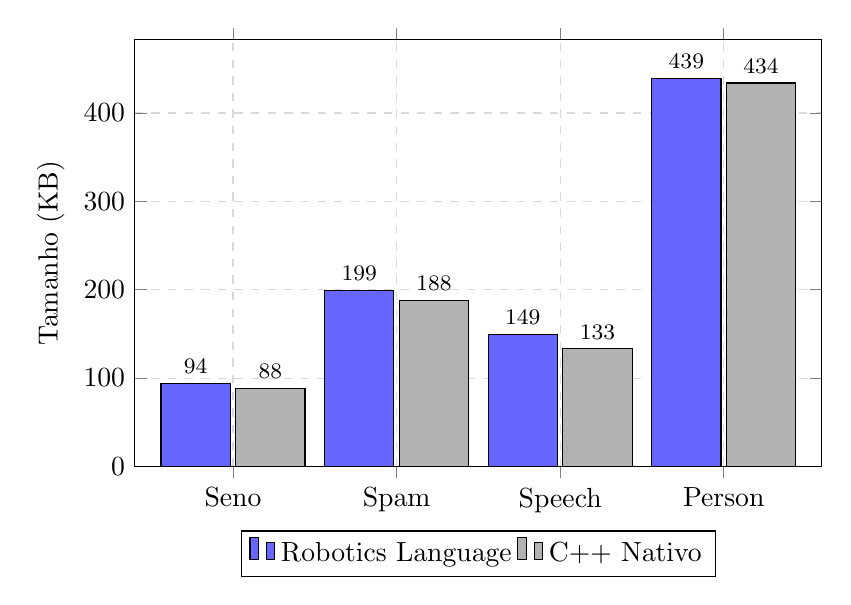
\begin{tikzpicture}
        \begin{axis}[
            ybar,
            symbolic x coords={Seno, Spam, Speech, Person},
            xtick=data,
            nodes near coords,
            nodes near coords style={font=\footnotesize},
            ylabel={Tamanho (KB)},
            xlabel={Modelos},
            legend style={at={(0.5,-0.15)}, anchor=north, legend columns=-1},
            width=0.85\textwidth,
            height=7cm,
            ymin=0,
            bar width=25pt,
            enlarge x limits=0.2,
            grid=major,
            grid style={dashed, gray!30}
        ]
            \addplot[fill=blue!60] coordinates {(Seno,94) (Spam,199) (Speech,149) (Person,439)};
            \addplot[fill=gray!60] coordinates {(Seno,88) (Spam,188) (Speech,133) (Person,434)};
            \legend{Robotics Language, C++ Nativo}
        \end{axis}
    \end{tikzpicture}
    \caption{Comparativo do tamanho do binário final (\textit{Flash}) entre as implementações.}
    \label{graf:tamanho-binario}
\end{figure}


Com base nos resultados apresentados, observa-se que a utilização da biblioteca padrão em RL introduz um \textit{overhead} natural devido à camada de abstração e ao \textit{wrapper} de compatibilidade. O aumento absoluto variou entre 5 KB e 16 KB.

No entanto, conforme ilustrado na \hyperref[graf:tamanho-binario]{Figura~\ref*{graf:tamanho-binario}}, esse impacto se torna menos significativo em aplicações maiores. No modelo \textit{Person Detection}, o maior testado, a diferença de 5 KB representou um aumento de apenas 1,15\% ($439$ KB contra $434$ KB), demonstrando que, para aplicações reais de maior porte, o impacto no armazenamento é aceitável.

\subsection{Análise do Tempo de Execução}
A \hyperref[notebook-tempo]{Tabela~\ref*{notebook-tempo}} exibe o tempo de execução médio obtido em cada teste.

\begin{table}[H]
\centering 
\caption{Tempo de execução (ms) na máquina de desenvolvimento}
\label{notebook-tempo}
    \begin{tabular}{cccc}
    \toprule
    \textbf{Modelo TinyML} & \textbf{Biblioteca padrão} & \textbf{TFLM(C++)}  \\ \midrule
    Preditor de Seno quantizado & 1.921 & 1.007 \\ 
    Preditor de Seno & 1.916 & 0.985 \\
    Classificador de Spam & 1.973 & 1.058 \\ 
    Micro Speech & 10.914 & 9.851 \\
    Person Detection - & 150.674 & 149.260 \\
    \bottomrule
    
    \end{tabular}
\end{table}

Nota-se um comportamento constante em todos os modelos testados: a diferença absoluta variou minimamente entre 0,914 ms e 1,414 ms. Isso indica um custo fixo de processamento introduzido pelo \textit{wrapper}. Para facilitar a visualização desse impacto em diferentes escalas, os resultados foram divididos em dois gráficos.

A \hyperref[graf:tempo-leves]{Figura~\ref*{graf:tempo-leves}} apresenta os modelos de baixa carga computacional. Nesses casos, o \textit{overhead} fixo é visualmente perceptível e representa uma parcela significativa do tempo total, chegando a dobrar o tempo em inferências muito rápidas (< 2 ms).

\begin{figure}[H]
    \centering
    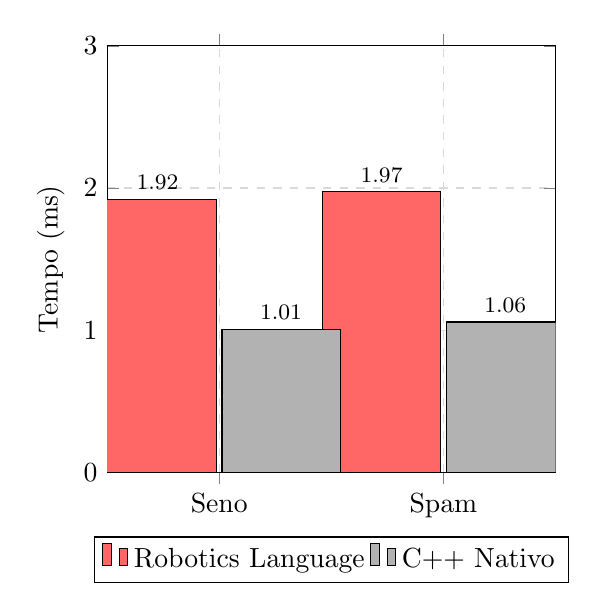
\begin{tikzpicture}
        \begin{axis}[
            ybar,
            symbolic x coords={Seno, Spam},
            xtick=data,
            nodes near coords,
            nodes near coords style={font=\footnotesize},
            ylabel={Tempo (ms)},
            xlabel={Modelos},
            ymin=0, ymax=3.0, 
            legend style={at={(0.5,-0.15)}, anchor=north, legend columns=-1},
            width=0.6\textwidth, % Menor largura pois tem poucas barras
            height=7cm,
            bar width=1.5cm, 
            enlarge x limits=0.5,
            grid=major,
            grid style={dashed, gray!30}
        ]
            \addplot[fill=red!60] coordinates {(Seno,1.921) (Spam,1.973)};
            \addplot[fill=gray!60] coordinates {(Seno,1.007) (Spam,1.058)};
            \legend{Robotics Language, C++ Nativo}
        \end{axis}
    \end{tikzpicture}
    \caption{Comparativo de tempo de execução para modelos leves (baixa carga computacional).}
    \label{graf:tempo-leves}
\end{figure}

Por outro lado, a \hyperref[graf:tempo-complexos]{Figura~\ref*{graf:tempo-complexos}} demonstra o comportamento em modelos mais complexos. É possível observar que a diferença visual entre as barras praticamente desaparece.

\begin{figure}[H]
    \centering
    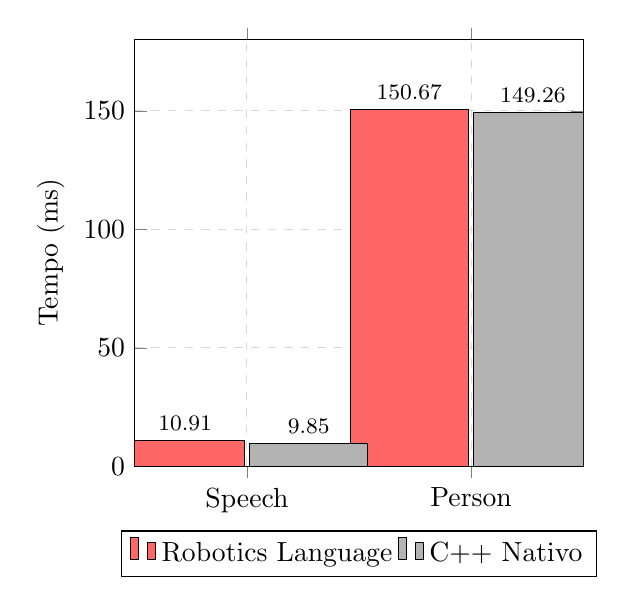
\begin{tikzpicture}
        \begin{axis}[
            ybar,
            symbolic x coords={Speech, Person},
            xtick=data,
            nodes near coords,
            nodes near coords style={font=\footnotesize},
            ylabel={Tempo (ms)},
            xlabel={Modelos},
            ymin=0, ymax=180, 
            legend style={at={(0.5,-0.15)}, anchor=north, legend columns=-1},
            width=0.6\textwidth,
            height=7cm,
            bar width=1.5cm,
            enlarge x limits=0.5,
            grid=major,
            grid style={dashed, gray!30}
        ]
            \addplot[fill=red!60] coordinates {(Speech,10.914) (Person,150.674)};
            \addplot[fill=gray!60] coordinates {(Speech,9.851) (Person,149.260)};
            \legend{Robotics Language, C++ Nativo}
        \end{axis}
    \end{tikzpicture}
    \caption{Comparativo de tempo de execução para modelos complexos.}
    \label{graf:tempo-complexos}
\end{figure}

Para o modelo \textit{Person Detection}, a diferença representa apenas cerca de 0,94\% do tempo total de execução (150,674 ms contra 149,260 ms). Isso confirma que o impacto relativo do \textit{wrapper} diminui drasticamente conforme a complexidade do modelo aumenta, tornando a solução viável para aplicações reais de TinyML.

\subsection{Análise Qualitativa: Facilidade e Manutenibilidade}

Além das métricas de desempenho, a facilidade de desenvolvimento e a manutenibilidade do código são fatores cruciais. Uma comparação pode ser feita entre o \hyperref[lst:teste-bib-rob]{Código~\ref*{lst:teste-bib-rob}} (\texttt{.rob} com biblioteca padrão) e \hyperref[lst:teste-cpp]{Código~\ref*{lst:teste-cpp}} (C++ com TFLM) apresentados nos apêndices do trabalho.

No desenvolvimento em C++, o programador precisa ter conhecimento detalhado da arquitetura do \textit{framework} para que consiga manipular corretamente os símbolos e funções do TFLM. Para que seja desenvolvida uma aplicação funcional é necessário: incluir múltiplos arquivos de cabeçalho específicos, instanciar manualmente o registrador de operadores e registrar operador por operador, gerenciar explicitamente o ciclo de vida do intérprete e a alocação de tensores, realizar verificações de versão de schema (TFLITE\_SCHEMA\_VERSION), acessar ponteiros brutos e iterar sobre eles para manipular os dados de entrada e saída, entre outras tarefas complexas.

Em contrapartida, o desenvolvimento utilizando a biblioteca padrão em RL é significativamente mais simples e direto. Com uma única linha de importação da biblioteca \texttt{ai.tflm}, o programador tem acesso a todas as funcionalidades necessárias para criar uma aplicação TinyML. O registro de operadores (\textit{kernels}) é feita de forma declarativa através de um array de IDs, eliminando a necessidade de chamadas de função repetitivas. Além disso, na inicialização do modelo, o processo de configuração do intérprete e alocação de tensores é abstraído, permitindo que o desenvolvedor foque apenas na lógica da aplicação. A manipulação dos dados de entrada e saída é realizada de maneira intuitiva, utilizando arrays nativos da RL, sem a necessidade de lidar com ponteiros brutos ou estruturas complexas.

Apesar do código em RL possuir mais caracteres por conta da ausência de um sistema de arquivos para incluir os dados do modelo e dados de entrada diretamente (como é feito em C++), o número de linhas de código é significativamente menor, o que facilita a leitura e manutenção do código.

